% !TeX program = xelatex
% Locality Causes Tractability? — arXiv preprint source
% Build: tectonic main.tex (XeTeX engine; reruns automatically for cross-references)
\documentclass[11pt]{article}
\usepackage[margin=1in]{geometry}
\usepackage{amsmath,amssymb}
\usepackage{booktabs}
\usepackage{graphicx}
\usepackage[hidelinks]{hyperref}
\hypersetup{pdftitle={Locality Causes Tractability? An Intervention Study on
the Variable-Interaction Radius in Geometric Random Satisfiability},
pdfauthor={Song Jin}}
\usepackage{microtype}
\usepackage{enumitem}
\setlist{topsep=2pt,itemsep=1pt}

\newcommand{\ac}[1]{\ensuremath{\alpha_c(#1)}}

\title{Locality Causes Tractability? An Intervention Study on the\\
Variable-Interaction Radius in Geometric Random Satisfiability}
\author{Song Jin\\
\small Independent Researcher\\\texttt{j.song.cs@outlook.com}}
\date{September 2026\\
\small \textbf{Compact Version} --- a full journal version is in preparation.}

\begin{document}
\maketitle

\begin{abstract}
A widespread intuition holds that real-world computational problems are easy
because their ``causes act locally'': when variables interact only within small
neighbourhoods, constraint solvers should scale well. Observational evidence
supports the intuition, but observation cannot separate locality from the many
other regularities real instances carry. We translate the intuition into a
falsifiable, interventional claim: holding the number of variables
fixed, matching clause density relative to each radius's own threshold, and
with clause-content statistics r-invariant by construction, varying
\emph{only} the radius $r$ within which clause variables are drawn from a 2-D
torus should causally change CDCL solving difficulty. Three findings.
\emph{(i)}~The operational satisfiability boundary is not $r$-invariant: it
lies below density 2.5 at $r=0.06$ and near the classical ${\approx}4.3$
region by $r=0.22$ (a displacement of at least 1.7 density units) ---
locality moves the sat/unsat boundary itself --- before becoming unmeasurable
at $r\ge 0.3$ under a $10^7$-conflict budget. \emph{(ii)}~At density matched relative to each
radius's own threshold, difficulty spans $3.4$ orders of magnitude across $r$
among decided instances (mean $\log_{10}$ conflicts $1.45 \to 4.86$ from
$r=0.06$ to $0.22$), and $\ge 4.5$ orders when budget-censored runs are
counted at their lower bound; RM-ANOVA $F(8,216)=2808.5$, $p\approx10^{-213}$;
Jonckheere--Terpstra $p\le 10^{-4}$ with FDR $q\le 10^{-4}$; partial
$\eta^2 \approx 0.99$. \emph{(iii)}~A degree-preserving swap that destroys
spatial locality while keeping every literal's occurrence count exactly fixed
raises difficulty by $16$--$68\times$ (Wilcoxon $p\le 7\times10^{-10}$) and
flips the satisfiability status of 53 instance pairs; causal mediation
attributes ${\sim}94\%$ of the radius effect to community-structure
restructuring (ACME 3.06, bootstrap CI $[2.84, 3.37]$). Locality is not merely
correlated with tractability --- under our controls it is the causal channel.
All claims are scoped to $n=400$, direct CNF encodings, and CDCL-family
solvers; we discuss what this does and does not say about P versus NP. Code,
seeds, data, preregistration, and the full audit trail are public.
\end{abstract}

\section{Introduction}
\label{sec:intro}

\paragraph{The conjecture and its observational gap.}
In popular discussions of \textsc{P} versus \textsc{NP}, one encounters a
philosophical diagnosis: problems resist algorithmic solution when variable
interactions are strongly correlated at long range; the computational world is
tractable because causation is local. As stated, the claim is unfalsifiable
--- ``locality'', ``correlation'', and ``cause'' are unoperationalized. Yet the
intuition has an empirically serious core. Industrial SAT instances --- the
reason conflict-driven clause-learning (CDCL) solvers~\cite{marques2009}
routinely decide formulas with millions of variables from competition and
application repositories~\cite{satcomp} --- exhibit community structure, small
backdoors, and heavy-tailed variable-incidence patterns. Observationally,
structure and ease co-occur.

Observation, however, cannot license a causal reading. Instances that are easy
and local are also many other things. The literature's own cautionary results
make the point sharp. Zulkoski et al.~\cite{zulkoski2018}, in the largest
correlational study to date (${\sim}7000$ competition instances), found that
\emph{no single} structural parameter significantly predicts CDCL runtime
across heterogeneous benchmark sets; the best six-feature regression reaches
adjusted $R^2 \approx 0.31$ on application instances, and the
size-plus-treewidth feature set reaches only $0.05$. Mull, Fremont and Seshia~\cite{mull2016} prove that
any ``polynomial-clique'' community metric --- including modularity --- admits
instances with excellent scores that remain \textsc{NP}-hard, and that
pseudo-industrial community-attachment instances require exponentially long
resolution proofs with high probability when communities are few. Structure,
by itself, neither certifies nor explains tractability.

\paragraph{What an intervention adds.}
The remedy is standard in the empirical sciences and rare in SAT difficulty
research: hold everything else fixed and turn one knob. We operationalize the
locality conjecture as a dose--response experiment. A \emph{locality-kernel
generator} samples each clause's variables uniformly from an $r$-ball on a
discrete 2-D torus and draws polarities from a standardized content
distribution whose statistics are $r$-invariant by construction
($\sigma$-redundancy histograms identical across $r$ in pilots); literal-degree
means equal $3\alpha$ exactly, varying across $r$ only through the
threshold-matched density $\alpha$, and the intervention arm's
degree-preserving swap holds the degree profile exactly fixed. The knob $r$ has a physical
reading: it is the \emph{spatial span of variable interaction} --- the exact
quantity the philosophical conjecture is about.

\paragraph{Contributions.}
\begin{enumerate}
\item \textbf{The first controlled intervention scan of locality radius.}
Nine $r$ levels $\times$ three preregistered offsets $\Delta$ above each radius's
\emph{own} operational threshold $\ac{r}$ (a fourth, $\Delta{=}{+}0.6$, at 4 of
the 9 radii; $r{=}0.06$ anchors are the lattice-nearest S0 grid value 2.6 (the
grid brackets the true boundary below 2.5) --- conservative
for the span) $\times$ 30 paired seeds $\times$ two
solvers, with per-instance structural metrics (treewidth bracketed by min-fill
upper and degeneracy lower bounds; modularity, community metrics, spectral
gap).
\item \textbf{A threshold curve $\ac{r}$} (832 solves at $10^7$-conflict
budget): the operational threshold is not $r$-invariant --- the boundary lies below
2.5 at $r=0.06$ and near ${\approx}4.3$ by $r=0.22$, before difficulty
saturates beyond measurable range at $r\ge0.3$; the \emph{measurability
boundary itself} tracks $r$.
\item \textbf{A structure-destruction intervention (E3b).} A degree-preserving
swap chain destroys spatial locality while keeping the literal degree sequence
exactly fixed; paired Wilcoxon tests isolate the causal contribution of
spatial structure.
\item \textbf{Topology $\times$ content decomposition}, with the content arm's
operationalization registered openly as an amendment (AMEND-3) rather than
shipped ill-defined.
\item \textbf{An honest negative-result protocol}: preregistration frozen
before the main scan, numbered amendments, a prespecification-vs-implementation
audit that caught one material bug before unblinding, and quantitative
triggers under which we would have reported ``density dominates''.
\end{enumerate}

\paragraph{Scope.}
All claims concern CDCL-family solvers on direct CNF encodings at $n=400$ with
conflict-count difficulty. We make no claim about \textsc{P} versus
\textsc{NP} (\S\ref{sec:discussion}). Machine-independence is obtained by
using conflict counts, not wall-clock, as the primary measure.

\section{Related Work}
\label{sec:related}

\paragraph{Structural measures and CDCL performance.}
Ans\'otegui et al.\ introduced the scale-free (power-law) variable-incidence
model of industrial-like instances~\cite{ansotegui2009}, later extended with
fractal-dimension analyses of incidence graphs (Ans\'otegui et al.\ 2014, as
tabulated in~\cite{zulkoski2018}); Newsham et al.~\cite{newsham2014} reported encouraging runtime regressions on
community features. Zulkoski et al.~\cite{zulkoski2018} scaled the design to
${\sim}7000$ instances from SAT Competitions 2007--2016 with MapleCOMSPS
runtimes and OLS/ridge regression over standardized features with full
pairwise interactions. Their findings anchor our baseline expectations:
no single parameter is significantly predictive in the aggregate; best
combos reach adjusted $R^2 \approx 0.31$ (application), $0.56$ (crafted),
$0.66$ (random); the size-plus-treewidth feature set carries almost no
explanatory power on application instances (adjusted $R^2 \approx 0.05$);
sub-category correlations are strong but \emph{sign-flipping}
(e.g.\ a mergeability ratio: Spearman $+0.94$ on argumentation, $-0.73$ on
hardware); and pre-simplification plus corpus grouping materially change
$R^2$ --- a sensitivity we inherit and control by reporting both calibers.
On the behavioral side, Zulkoski et al.\ show CDCL branching (VSIDS, LRB) is
spatially local with respect to variable-incidence-graph communities (Gini
$0.50$--$0.52$ vs $0.16$ for random branching) and temporally local (45--55\%
of decisions land in the most recent 1\% of communities). Li et
al.~\cite{li2022} document the hierarchical community structure of practical
instances.

\paragraph{Locality and heterogeneity: theory.}
Bl\"asius et al.~\cite{blasius2022} prove that heterogeneity alone does not
make random $k$-SAT easy (superpolynomial resolution size), whereas geometric
locality yields small unsatisfiable subformulas findable in polynomial time ---
the strongest existing theorem-level support for ``locality $\Rightarrow$
tractability'', and the regime map our generator navigates. Gir\'aldez-Cru
and Levy's locality-based generator variants~\cite{giraldez2017};
Mull et al.~\cite{mull2016} then proved average-case hardness for
community-attachment instances with few communities, and showed
experimentally that \emph{community size, not formula size, dominates
runtime}: instances differing $55\times$ in variables but matched in community
size differ ${\sim}3\times$ in runtime --- an observational precursor of our
interventional question. Jia, Moore and Strain~\cite{jia2005} analyze planted
SAT via solution hiding; their planting threshold is consistent with naive planted
ensembles being CDCL-trivial, a pilot finding that motivated our non-planted
difficulty carrier.

\paragraph{Proof complexity: the width backbone.}
Atserias and Dalmau~\cite{atserias2008} characterize resolution width
combinatorially, yielding $w(F\vdash\bot) \ge \mathrm{tw}(\text{primal}) - 2$
for 3-CNFs.
Ben-Sasson and Wigderson~\cite{ben1999} relate width to size,
$S \ge \exp(\Omega((w-w_0)^2/n))$: a ``width barrier'' at
${\approx}\sqrt{n\log n}$. Atserias--Fichte--Thurley~\cite{atserias2011} and
Beame et al.~\cite{beame2003} connect CDCL to (bounded-width) resolution.
Together: low treewidth $\Rightarrow$ short proofs exist $\Rightarrow$
CDCL with restarts finds them in polynomial time --- the theoretical face of
our E1 result (width-controlled instances are flat and trivial at all $k$).
Correlation decay~\cite{weitz2006} and the overlap-gap property
(see~\cite{gamarnik2021}) delineate where local information provably suffices
or fails; we use these as interpretive scaffolding only, since practical CDCL
carries components outside these models.

\section{Problem Setup and Instance Generators}
\label{sec:setup}

\paragraph{Locality kernel (\texttt{geo\_random}).}
Fix $n=400$ variables placed uniformly on a discrete 2-D torus of side
$\sqrt{n}$. Each of $m=\alpha n$ clauses: pick a centre uniformly, collect the
variables within torus distance $r$ (up to 1000 attempts to find a ball
containing at least three variables), sample 3 distinct variables from that
ball, and draw polarities uniformly
(\texttt{planted=False}). Small $r$ gives high intra-cluster variable reuse
and sparse inter-cluster coupling; $r\to\infty$ recovers approximately uniform
random 3-SAT. Because the torus diameter is ${\sqrt{2}}/{2}\approx0.71$, the
$r{=}0.8$ and $r{=}1.5$ levels (whose $r$-ball spans all $n$ variables)
generate identical clause sets; sensitivity analyses treat them as one level.
A \emph{planted} variant draws polarities from
$\sigma$-satisfaction modes built on a global assignment $\sigma$: for the
$k$ positions a clause satisfies $\sigma$ on, a cardinality is drawn uniformly
in $1\ldots k$ and then a subset of that cardinality; a decoy assignment
$\beta$ instead constrains the fill of the hidden clause fraction (the
$q_{\text{hidden}}<1$ arm). Clause-content statistics are therefore
$r$-invariant by construction: redundancy histograms are identical across $r$
(verified in pilots; measured mean $\sigma$-redundancy ${\approx}2.2$).

\paragraph{Width-controlled family.}
$k$-tree skeletons give constructive treewidth $\le k$; matched random
families at the same $(n,\alpha)$ provide controls. Planted and unplanted arms
separate ``having a solution planted'' from ``being structured''.

\paragraph{Structure-destruction intervention (E3b).}
A bipartite swap chain (MCMC edge swaps on the variable--clause incidence
graph, rejecting swaps that duplicate a variable in a clause or create
complementary-literal pairs) destroys spatial locality while preserving every
literal's degree \emph{exactly}. The swapped instance is not a draw from the
\texttt{geo\_random} distribution; per our preregistration we report it as a
structure-destruction intervention, and record solver-status flips per pair
explicitly.

\paragraph{Topology $\times$ content factorial.}
The topology channel is original vs.\ swapped incidence graph. The content
channel's unambiguous operationalization on our unsatisfiable-arm carrier is
non-trivial (a distribution-preserving polarity resample is the identity by
construction there); we registered this tension openly as AMEND-3 and deferred
the interaction test rather than shipping an ill-defined arm. The topology
channel is fully executed (E3b).

\paragraph{Threshold matching.}
Difficulty near threshold is U-shaped in density, so comparing arms at fixed
absolute $\alpha$ confounds $r$-effects with threshold proximity. A dedicated
threshold study (S0, \S\ref{sec:s0}) estimates the operational threshold
$\ac{r}$ per radius; the main scan samples at $\alpha = \ac{r} + \Delta$,
$\Delta \in \{+0.2, +0.4, +0.8\}$.

\section{Measures, Solvers, and Statistical Protocol}
\label{sec:method}

\paragraph{Difficulty.}
Primary: $\log_{10}(\text{conflicts}+1)$ under CaDiCaL, conflict budget
$10^6$ (main scan) / $10^7$ (threshold study). CaDiCaL's budget mechanism
counts decided conflicts precisely, giving machine-independent censoring.
Secondary: wall-clock (same machine), Glucose cross-checks. A 300\,s
subprocess-isolated wall guard returns status \textsc{walltimeout} for runs
where conflicts are sparse but propagation explodes; these rows carry no
conflict count, are excluded from conflict analyses and from the
Kaplan--Meier estimation (their censored-mass trend is reported separately,
\S\ref{sec:e3a}); their directional bias is declared (AMEND-2):
truncation falls disproportionately on the \textsc{unsat} side near
threshold, which \emph{raises} resolved-SAT rates and pushes $\ac{r}$ upward
--- an anti-conservative bias for our gradient hypothesis, bounded by
spot-checks at $10^8$ conflicts / 480\,s on flagged radii
(\S\ref{sec:threats}).

\paragraph{Structural measures.}
Treewidth is reported as a bracket: min-fill upper bound (validated against
$k$-tree constructions) and degeneracy-based lower bound. Community structure
(Leiden, fixed resolution), modularity, spectral gap, redundancy histograms;
all metrics are computed deterministically on the generated instance and
stored with it.

\paragraph{Statistics.}
Repeated-measures ANOVA with seed as subject (seeds shared across all
$r\times\Delta$ cells), partial $\eta^2 = F\cdot df_1/(F\cdot df_1+df_2)$;
Jonckheere--Terpstra ordered-alternative test by Monte Carlo permutation;
paired Wilcoxon signed-rank for E3b pairs; Tobit (type-I, right-censored) and
Kaplan--Meier as censoring analyses; Imai et al.~\cite{imai2011} causal mediation
(product-of-coefficients estimator) with bootstrap percentile ACME confidence
intervals; Benjamini--Hochberg FDR across the
primary family. Decision rules were preregistered: H2 confirmed by
FDR-corrected $p<0.05$ with partial $\eta^2 \ge 0.14$ or $\ge 10\times$
median endpoint ratio; ``density dominates'' triggered by $\eta^2<0.02$ and
$p>0.05$.

\paragraph{Preregistration and audit.}
Hypotheses, censoring semantics, $r$ levels, and decision rules were frozen
before the main scan. Amendments are numbered and reason-stated: AMEND-1 (S0
budget $10^7$), AMEND-2 (wall guard, bias declaration, spot-check protocol),
AMEND-3 (content-arm deferral). A prespecification-vs-implementation audit
records every deviation found by item-by-item inspection --- including one
material bug (walltimeout rows initially counted as \textsc{unsat} in
threshold estimation) fixed \emph{before} the main scan fired.

\section{Results I: The Threshold Curve \texorpdfstring{$\ac{r}$}{alpha\_c(r)} (S0)}
\label{sec:s0}

S0 resolves 832 runs (720 preregistered grid jobs + 112 grid-floor extension
jobs) at $10^7$-conflict budget, 16 seeds per cell. With only resolved runs
contributing to SAT rates (AMEND-2 caliber) and linear interpolation of the
$0.5$-crossing (Fig.~\ref{fig:alphac}):

\begin{table}[h]
\centering
\begin{tabular}{lccccccccc}
\toprule
$r$ & 0.06 & 0.08 & 0.11 & 0.15 & 0.22 & 0.3 & 0.5 & 0.8 & 1.5\\
\midrule
$\ac{r}$ & $<2.5^{\dagger}$ & 3.35 & 3.82 & 4.20 & 4.23 & 4.40$^{*}$ & 4.70$^{*}$ & 4.60$^{*}$ & 4.60$^{*}$\\
censoring & 2.1\% & 0\% & 0\% & 0\% & 0\% & 92.5\% & 98.8\% & 100\% & 100\%\\
\bottomrule
\end{tabular}
\caption{Operational threshold vs.\ locality radius. $^{*}$measurement-saturated
radii: the crossing is unidentifiable; the table carries the pilot coarse
value, flagged low-confidence, with spot-checks per AMEND-2. $^{\dagger}$the
SAT rate never reaches 0.5 on the explored grid ($\alpha\in[2.5,3.1]$, rate
${\sim}0.31$ at the grid floor declining to ${\sim}0.13$): the boundary at
$r=0.06$ is bracketed from above, not pinpointed.}
\label{tab:alphac}
\end{table}

\begin{figure}[t]
\centering
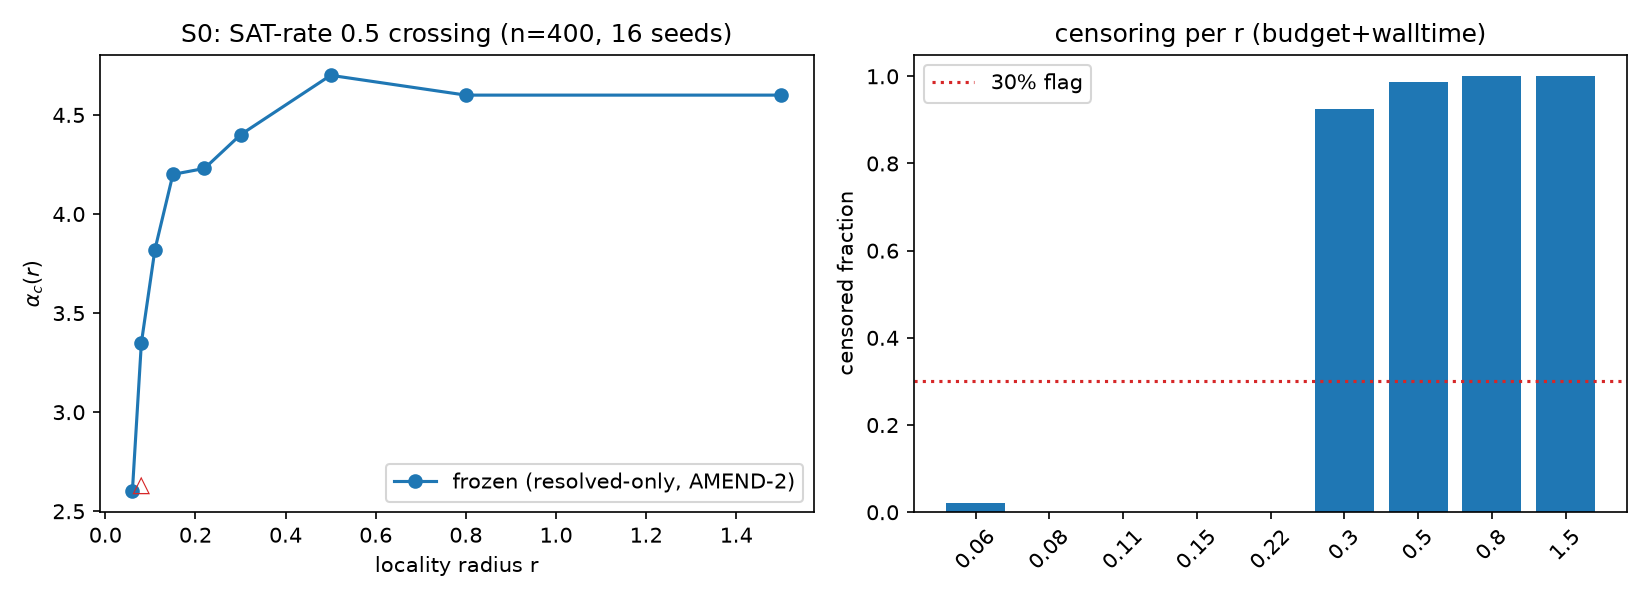
\includegraphics[width=0.85\linewidth]{figures/fig_s0_alphac.png}
\caption{Left: the operational threshold $\ac{r}$, resolved-only caliber
(AMEND-2; $\triangle$ marks radii whose grid has no $0.5$-crossing, carried at
their lattice-nearest pilot values). Right: censoring fraction per radius
(budget + walltime) --- the measurability boundary itself tracks $r$.}
\label{fig:alphac}
\end{figure}

Three observations. \emph{(i)}~The operational threshold is not
$r$-invariant. At $r=0.06$ the SAT rate is already only ${\sim}0.31$ at
density 2.5 and declines gently through 3.1 (censoring $\le2.1\%$): the
boundary is bracketed below density 2.5. By $r=0.22$ it has risen past 4.2
--- a displacement of \emph{at least} 1.7 density units. Locality does not
merely re-scale difficulty around a fixed threshold, it \emph{moves the
threshold itself}. \emph{(ii)}~The curve saturates near the classical
random-3-SAT threshold region ($\alpha_c \to 4.267$ as $n\to\infty$),
consistent with $r\to\infty$ recovering uniform random 3-SAT and with the
width-backbone picture: small radii admit satisfiability far below it (the
geometric small-subformula regime of~\cite{blasius2022}). \emph{(iii)}~At $r\ge0.3$,
near-threshold instances collapse out of measurable range (313 walltimeouts
concentrated there): the question ``where is the threshold'' stops being
answerable at fixed budget --- a difficulty-regime change, bounded by
spot-checks (\S\ref{sec:threats}).

\section{Results II: Dose--Response at Matched Threshold Offset (E3a)}
\label{sec:e3a}

The main scan places 9 radii $\times$ 3 offsets above each radius's own
$\ac{r}$, 30 paired seeds, two solvers. 1980 runs, zero errored rows; 1436
resolved, 544 censored (27.5\%, concentrated at $r\ge0.3$). Figure~\ref{fig:dose}
visualizes both arms.

\paragraph{Primary tests (CaDiCaL, $\Delta$-pooled, seeds as subjects).}
RM-ANOVA on the $\Delta$-aggregated complete-seed subset ($\Delta\in\{0.2,
0.4,0.6,0.8\}$, the $0.6$ arm present at 4 of the 9 radii; $n=28$ seeds
observed at all radii): $F(8,216)=2808.5$, $p\approx1.1\times10^{-213}$.
Jonckheere--Terpstra (Monte Carlo permutation, $10^4$ draws): $p\le10^{-4}$
--- the resolution floor of the permutation distribution --- for every
$(\Delta, \text{solver})$ cell; BH-FDR $q \le 10^{-4}$ across the seven-member
primary family. A censoring-robust variant (censored runs scored at the
budget value) reproduces $p\le10^{-4}$, so the trend is not an artifact of
dropping censored rows. Kaplan--Meier curves of time-to-decision
(Fig.~\ref{fig:km}) make the same point visually: the median conflict count at
decision rises from 23 ($r=0.06$; identical under the Kaplan--Meier
estimator) through 20{,}695 ($r=0.22$, Kaplan--Meier median) to censoring
plateaus --- half or more undecided at $r\ge0.5$, about a quarter at $r=0.3$.

\begin{table}[h]
\centering
\begin{tabular}{lccccccc}
\toprule
$r$ & 0.06 & 0.08 & 0.11 & 0.15 & 0.22 & 0.3 & 0.5\\
\midrule
mean $\log_{10}$ conflicts & 1.45 & 1.68 & 2.30 & 3.02 & 4.86 & 5.87$^{*}$ & 5.93$^{*}$\\
resolved $n$ & 30 & 30 & 30 & 30 & 30 & 9/30 & 2/30\\
\bottomrule
\end{tabular}
\caption{Dose--response at $\Delta=+0.2$ (the near-threshold arm, CaDiCaL).
$^{*}$means over surviving (easier) instances only; the censoring-aware
Jonckheere--Terpstra bounds the underlying trend.}
\label{tab:dose}
\end{table}

\begin{figure}[t]
\centering
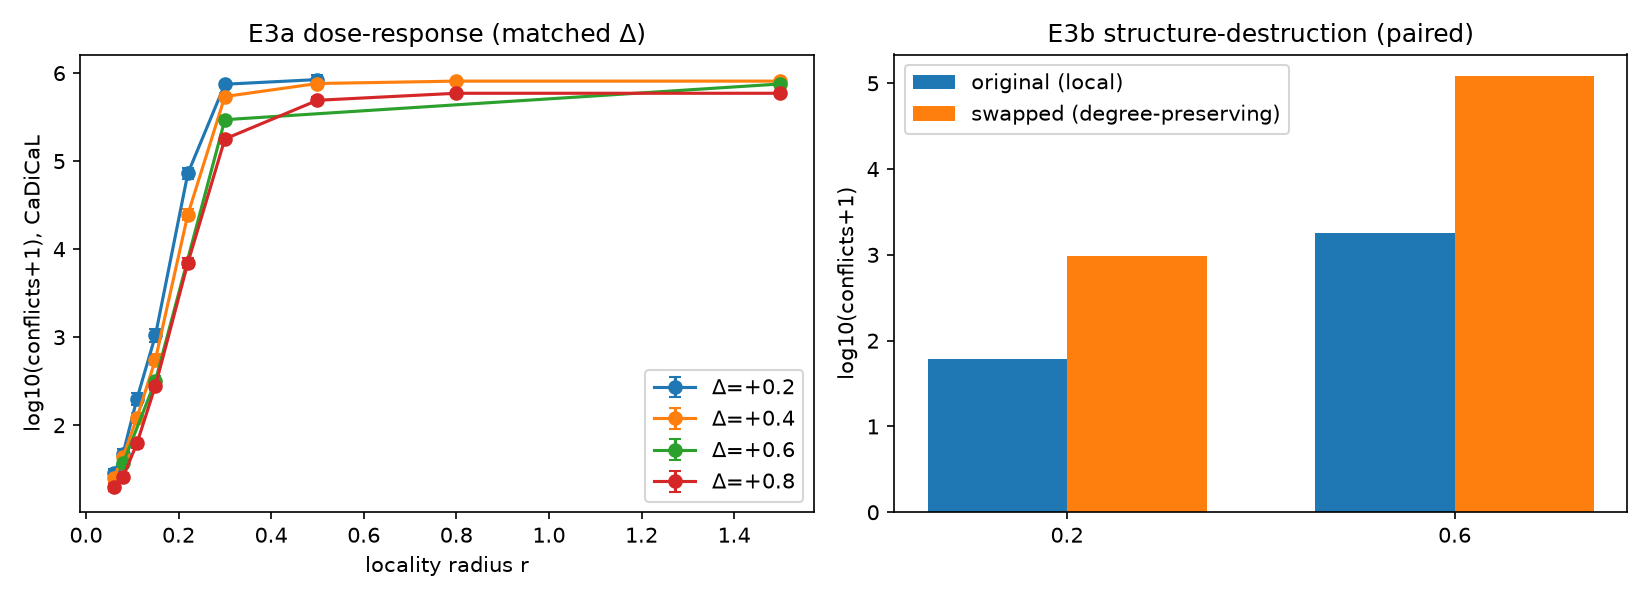
\includegraphics[width=0.95\linewidth]{figures/fig_e3a_dose.png}
\caption{Left: dose--response of difficulty to the locality radius at matched
threshold offsets (mean $\pm$ s.e.m., CaDiCaL; $\Delta{=}{+}0.8$ endpoints
$1.29$ at $r{=}0.06$ and $5.77$ at $r{=}0.8$). Right: paired
structure-destruction effect (E3b).}
\label{fig:dose}
\end{figure}

From $r=0.06$ to $r=0.22$ at the \emph{same} threshold offset, difficulty
climbs from ${\sim}28$ to ${\sim}72{,}000$ conflicts --- \textbf{3.4 orders of
magnitude} among decided instances, and $\ge 4.5$ orders when the censored
runs at $r\ge0.3$ are counted at their budget lower bound. The
$\Delta=+0.8$ arm repeats and extends the pattern ($1.29$ at $r{=}0.06$ $\to$
$5.77$ at $r{=}0.8$,
${\approx}4.5$ orders).
Partial $\eta^2$ at computable cells is $0.985$--$0.988$ against the
preregistered confirmation threshold of $0.14$, and the $\Delta=+0.8$ arm's
endpoint ratio ${\sim}10^{4.5}$ dwarfs the preregistered $10\times$ line. \textbf{H2 is
confirmed under its own preregistered decision rule.} Glucose replicates the
pattern.

\paragraph{$\Delta$ semantics under $\ac{r}$ bias.}
For flagged radii the $\alpha_c$ carries a bounded (and for $r\ge0.5$,
unbounded) overestimate (\S\ref{sec:threats}); this shifts the precise
horizontal placement of those cells but leaves the matched-comparison
structure --- within-$r$ across $\Delta$, within-$\Delta$ across $r$ ---
intact, which is where the gradient evidence lives.

\begin{figure}[t]
\centering
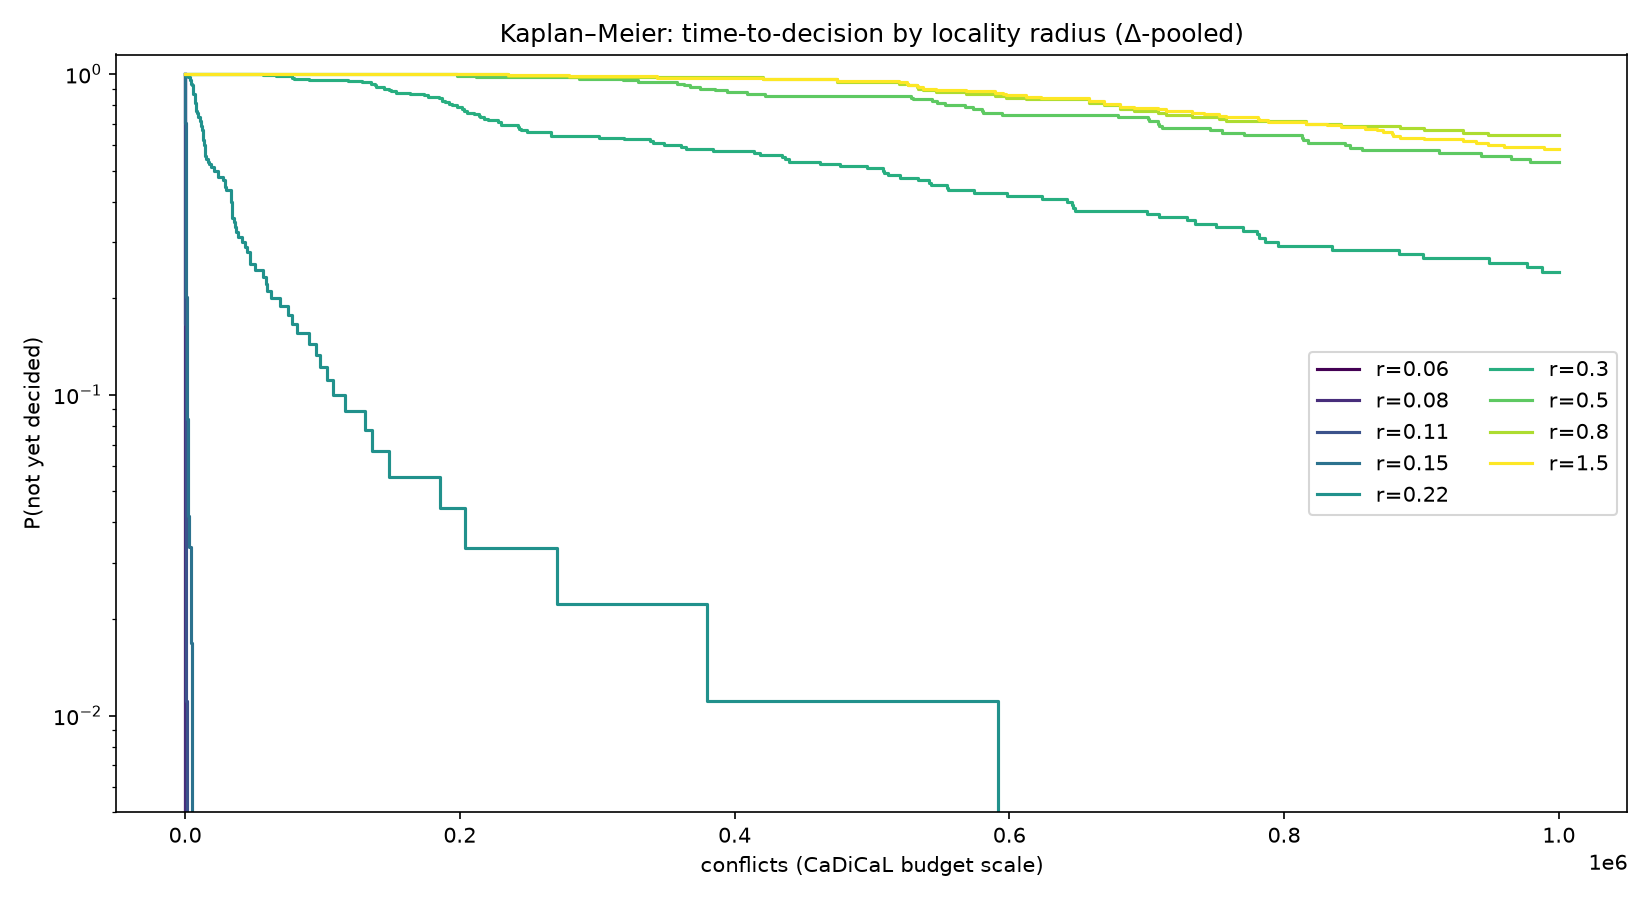
\includegraphics[width=0.9\linewidth]{figures/fig_km.png}
\caption{Kaplan--Meier estimates of time-to-decision (conflicts; CaDiCaL,
$\Delta$-pooled). Curves for small $r$ drop to zero within the budget; curves
for $r\ge0.5$ plateau at high ``not yet decided'' probability (about a
quarter at $r=0.3$) --- the
measurability boundary of \S\ref{sec:s0}, seen at the solver level.}
\label{fig:km}
\end{figure}

\section{Results III: The Structure-Destruction Intervention (E3b)}
\label{sec:e3b}

Degree-preserving swapping holds every literal's occurrence count \emph{exactly}
fixed while destroying spatial locality. Paired Wilcoxon signed-rank:

\begin{table}[h]
\centering
\begin{tabular}{lccccc}
\toprule
$\Delta$ & pairs & original mean logc & swapped mean logc & ratio & $p$\\
\midrule
$+0.2$ & 33 & 1.79 & 2.99 & $\times 16$ & $7.0\times10^{-10}$\\
$+0.6$ & 49 & 3.25 & 5.08 & $\times 68$ & $6.0\times10^{-13}$\\
\bottomrule
\end{tabular}
\caption{E3b paired results. 53 of the 82 resolved pairs flip satisfiability
status under the swap.}
\label{tab:e3b}
\end{table}

Together with E1 --- width-controlled instances are flat and trivial at all
$k$ (per-$k$ medians pooling both sizes, unplanted arm: $7$--$10$ conflicts
across $k\in\{3,5,8,12,16,20\}$, at $n\in
\{300,600\}$) --- the asymmetry is sharp: what CDCL difficulty responds to
is \emph{local geometry}, not any global topological summary.

\section{Results IV: Mediation and the Feature Ladder (H1)}
\label{sec:mediation}

Imai et al.~\cite{imai2011} causal mediation of the $r \to$ difficulty path (bootstrap
95\% CI; total effect 3.26 log units): modularity ACME $= 3.06\ [2.84, 3.37]$
(${\sim}94\%$ of total); spectral gap ACME $= 3.92\ [3.68, 4.28]$
(suppression: direct effect $-0.66$ --- evidence of a secondary channel
bypassing community structure); mean degree $2.34\ [2.15, 2.60]$; clustering
$2.19\ [2.02, 2.44]$. All CIs exclude zero: by the preregistered rule,
\textbf{mediation is established} as mechanism evidence.

The H1 feature ladder: on the main-scan data, ridge-CV $R^2$ rises from
$0.610$ (size features) and $0.664$ (size+density) to $\mathbf{0.976}$ with
structural features --- on controlled families, structure carries predictive
power that observation on random families cannot see (random-family baseline:
$0.90$ with zero structural gain). The preregistered nested OLS
$F$-test on the same subset confirms the ladder: $F(60,1283)=297.8$,
$p<10^{-4}$ for the structural block beyond size+density. A
gradient-boosted predictor with leave-one-$r$-out extrapolation (training
never sees the target radius) reaches $R^2 = 0.76$: structural features
generalize to unseen locality levels.

\section{Results V: Placement on Real Instances (E4-prime)}
\label{sec:e4}

All 59 fetched real instances (42 combinatorial/crafted from a public
benchmark suite; 17 DIMACS classics) were solved under the S0 budget protocol:
22/59 decided. The DIMACS classics anchor the easy end: 15 \textsc{sat} and 2
\textsc{unsat}, all decided within milliseconds (an audit caught a parsing
artifact in the 1996 legacy DIMACS dialect, silently truncating these files;
they were re-solved after the fix, with the full trail in the repository log).
The combinatorial challenge instances mostly exceed the wall guard (hard
anchor); file-name labels match our determinations on every checkable Heule
instance, though one legacy \texttt{-yes} file is in fact \textsc{unsat}. Our
generator's difficulty spectrum spans the middle of the real spectrum from
textbook-easy to competition-hard. The industrial-diversity caveat stands
(\S\ref{sec:threats}).

\section{Threats to Validity}
\label{sec:threats}

\paragraph{Construct.}
``Locality radius $r$'' is one spatial operationalization on a 2-D torus host;
other hosts and other notions may disagree. Our claim is about $r$ as defined.
Difficulty is conflict counts under CDCL --- a proxy for, not a definition of,
hardness.

\paragraph{Internal.}
Five controls close the confounding routes we identified: the variable count
$n$; the density $\alpha$ (fixed or $\Delta$-matched); the literal degree
profile (degree-cap rejection in the planted arms; \emph{exact} preservation
under the E3b swap --- the decisive control); the clause content (standardized
polarity sampling, $r$-invariant redundancy); and the solver engine (two
engines). Metrics are computed deterministically before solving, so the
metric-computation channel cannot pseudo-correlate with runtime. Censoring is
the residual internal threat: the wall guard is directionally biased
(AMEND-2), the direction was declared before unblinding, and spot-checks at
$10^8$ conflicts bound the $\alpha_c$ bias --- at $r=0.3$, \textsc{sat}
instances appear $0.2$ below the operational threshold (bias $\in[-0.2,0]$
density units); at $r\ge0.5$ $\pm0.2$ offsets fail to bracket the boundary at
$10^8/480$\,s --- every instance at $\alpha_c+0.2$ is decided \textsc{unsat}
while those at $\alpha_c-0.2$ stay undecided --- so the measurability boundary
is robust and the flagged $\alpha_c$ values carry an unbounded-bias caveat.
One material implementation
deviation was caught by the prespecification audit \emph{before} unblinding
and fixed; the trail is public.

\paragraph{Literal-degree profile.}
Because density is $\Delta$-matched to each radius's own threshold, the mean
literal degree ($3\alpha$: $8.4$ at $r=0.06$ vs.\ $14.7$ at $r=0.5$ in the
$\Delta{=}{+}0.2$ arms) necessarily co-varies with $r$ --- inherent to
threshold matching, and standardized by measuring density as a distance from
each radius's own boundary. The \emph{shape} of the literal-degree
distribution, however, is monitored rather than enforced in the main
\texttt{geo\_random} family: across the $\Delta{=}{+}0.2$ cells (30 seeds
each) its per-cell worst-case maximum degree spans $24$--$31$ (${\sim}29\%$
above the low-$r$ endpoint) across $r$, exceeding the ${<}5\%$ matching
criterion laid down in the frozen H2 premise, while the per-cell standard
deviation stays within it ($3.75 \to 3.85$, ${\sim}3\%$). We disclose this
deviation rather than silently incur it. It does not carry the causal
attribution, which rests on the E3b swap alone: that intervention preserves
the literal occurrence counts of every instance \emph{exactly}, so the
$16$--$68\times$ paired difficulty shift cannot be carried by degrees. We do
not lean on the direction of the residual shape drift, because the two tail
readings point opposite ways --- absolute tails grow toward the \emph{large}-$r$
end (where heavier tails are typically the \emph{easier} regime for CDCL),
while the relative dispersion falls (coefficient of variation ${\sim}0.45 \to
0.26$ across $r$), i.e.\ the small-$r$ end is the relatively heavier-tailed
one. Either reading leaves the causal claim unchanged. A degree-capped
\texttt{geo\_random} variant remains an open robustness arm.

\paragraph{External.}
\texttt{geo\_random} is an intervention vehicle, not a survey of practice;
the real-instance placement is restricted to decided instances, with the
industrial-diversity caveat documented (the canonical SAT 2024 main-track
files were unreachable from our network; the deterministic preselection table
--- 400 instances with hashes and 15-solver reference runtimes --- is retained
in the authors' working archive for future completion). All conclusions are scoped to CDCL-family solvers, direct CNF
encodings, $n=400$, and conflict-count difficulty.

\paragraph{Statistical conclusion.}
Paired designs with 30 seeds per cell, preregistered effect-size thresholds,
FDR over the primary family, and censoring-robust cross-checks.

\section{Discussion: What This Does and Does Not Say About P vs NP}
\label{sec:discussion}

Nothing we measure bears on \textsc{P} versus \textsc{NP}. The conjecture we
test descends from a philosophical \emph{intuition} about why the
computational world feels tractable --- ``causes act locally'' --- and
intuitions of this kind deserve attention precisely because they can be
operationalized and then shot down.

\paragraph{Phase transitions and a portable diagnostic.}
A classical observation --- dating to Cheeseman, Kanefsky and Taylor's
``Where the really hard problems are''~\cite{cheeseman1991} --- holds that
combinatorial problems are hardest near structural phase transitions. Our
results give that observation a \emph{causal, solver-relative} reading for
SAT/CDCL: the locality radius moves the transition itself and restructures
difficulty within matched offsets. The framework --- one structural knob,
threshold-matched dosing, a structure-destruction intervention,
censoring-aware statistics --- is offered as a \emph{portable diagnostic
protocol}: any claim of the form ``structural property $P$ helps algorithm $A$
on family $F$'' can be subjected to the same treatment. We explicitly do
\emph{not} claim our conclusions extend to local-search solvers; the contrast
is a preregistered prediction: if difficulty is a structure$\times$algorithm
relation, a stochastic local-search solver should respond to $r$ differently
--- possibly inversely --- and running it on our instances is a cheap,
decisive test.

\paragraph{Tractability is a relational property.}
E1 (width-controlled instances are flat) and the threshold curve together
suggest that difficulty lives neither in global topology alone nor in density
alone, but in the interaction between spatial organization and the search
dynamics of a particular algorithm family. CDCL branching is measurably
local~\cite{zulkoski2018}; our experiments ask whether the local geometry of
the \emph{instance} is what that locality feeds on. A ``yes'' makes the
philosophical conjecture precise enough to be useful; a ``no'' makes it
precise enough to be abandoned --- either outcome is progress over an
unfalsifiable slogan.

\paragraph{The measurability boundary is a finding.}
That near-threshold instances at $r\ge0.3$ collapse beyond our budgets is not
an inconvenience to be apologized for; it is the signature of a regime
change. Between $r=0.06$ (threshold bracketed cleanly at tiny budgets) and
$r=0.5$ (threshold invisible at $10^7$ conflicts), the \emph{character} of the
difficulty phase transition changes --- exactly what a locality-causal story
predicts, and what a density-only story has no reason to produce.

\paragraph{Intervention as a community practice.}
Structure--difficulty research has leaned on observational regression for two
decades --- with the field's own flagship study concluding that no structural
measure is strongly predictive of CDCL performance in the
aggregate~\cite{zulkoski2018}.
Intervention designs --- one knob, everything else pinned, preregistered
decision rules, censoring declared --- are the standard remedy in every
empirical science that has faced the same impasse. The generator, the swap
chain, the statistical protocol and the audit trail are released so that the
next conjecture can be tested the same way.

\section{Reproducibility Statement}
\label{sec:repro}

AI-assisted tools were used in data analysis and manuscript preparation (full
disclosure in the accompanying Zenodo snapshot, DOI: 10.5281/zenodo.22777748).

All instances are deterministically generated from
$(\text{family}, \text{params}, \text{seed})$ tuples; the result store keys
rows by $(\text{family}, \text{params}, \text{seed}, \text{solver})$ with
idempotent resume-per-row semantics; every figure regenerates from the SQLite
stores by committed scripts; result databases and manifests are
version-controlled. The full experiment matrix, budgets, the preregistration
with numbered amendments, and the prespecification-vs-implementation audit are
in the repository.

\begin{thebibliography}{18}\small

\bibitem{marques2009} J.~Marques-Silva, I.~Lynce, S.~Malik. Conflict-driven
clause learning SAT solvers. In \emph{Handbook of Satisfiability}, 2nd ed.,
FAIA 336 (2021). doi:10.3233/faia200987.

\bibitem{satcomp} SAT Competition series (2002--2026). Official archives and
results: \url{https://satcompetition.github.io/} (online resource).

\bibitem{li2022} C.~Li et al. On the hierarchical community structure of
practical Boolean formulas. \emph{SAT 2021}, LNCS 12831, pp.~359--376.
doi:10.1007/978-3-030-80223-3\_25; arXiv:2103.14992.

\bibitem{zulkoski2018} E.~Zulkoski, R.~Martins, C.~Wintersteiger, J.~Liang,
K.~Czarnecki, V.~Ganesh. The effect of structural measures and merges on SAT
solver performance. \emph{CP 2018}, LNCS 11008, pp.~436--452.
doi:10.1007/978-3-319-98334-9\_29.

\bibitem{mull2016} N.~Mull, D.~Fremont, S.~A. Seshia. On the hardness of SAT
with community structure. \emph{SAT 2016}, LNCS 9710, pp.~141--159.
doi:10.1007/978-3-319-40970-2\_10; arXiv:1602.08620.

\bibitem{ansotegui2009} C.~Ans\'otegui, M.~L. Bonet, J.~Levy. Towards
industrial-like random SAT instances. \emph{IJCAI 2009}. Companion:
\emph{On the structure of industrial SAT instances}, \emph{CP 2009},
pp.~127--141, doi:10.1007/978-3-642-04244-7\_13.

\bibitem{newsham2014} Z.~Newsham, V.~Ganesh, S.~Fischmeister, G.~Audemard,
L.~Simon. Impact of community structure on SAT solver performance.
\emph{SAT 2014}, LNCS 8561, pp.~252--268. doi:10.1007/978-3-319-09284-3\_20.

\bibitem{blasius2022} T.~Bl\"asius, T.~Friedrich, A.~G\"obel, J.~Levy,
R.~Rothenberger. The impact of heterogeneity and geometry on the proof
complexity of random satisfiability. \emph{SODA 2021}, pp.~42--53;
\emph{Random Structures \& Algorithms} 63(4):885--941 (2023).
doi:10.1002/rsa.21168.

\bibitem{giraldez2017} J.~Gir\'aldez-Cru, J.~Levy. Locality in random SAT
instances. \emph{IJCAI 2017}, pp.~638--644. doi:10.24963/ijcai.2017/89.

\bibitem{jia2005} H.~Jia, C.~Moore, D.~Strain. Generating hard satisfiable
formulas by hiding solutions deceptively. \emph{AAAI-05}, pp.~384--389.

\bibitem{atserias2008} A.~Atserias, V.~Dalmau. A combinatorial
characterization of resolution width. \emph{J.~Computer and System Sciences}
74(3):323--334. doi:10.1016/j.jcss.2007.06.025.

\bibitem{ben1999} E.~Ben-Sasson, A.~Wigderson. Short proofs are narrow ---
resolution made simple. \emph{J.~ACM} 48(2):149--169 (2001). doi:10.1145/375827.375835.

\bibitem{imai2011} K.~Imai, L.~Keele, D.~Tingley, T.~Yamamoto. Unpacking the
black box of causality: Learning about causal mechanisms from experimental
and observational studies. \emph{American Political Science Review}
105(4):765--789 (2011). doi:10.1017/S0003055411000414.

\bibitem{atserias2011} A.~Atserias, J.~K.~Fichte, M.~Thurley. Clause-learning
algorithms with many restarts and bounded-width resolution. \emph{JAIR} 40
(2011), pp.~353--373. doi:10.1613/jair.3152.

\bibitem{beame2003} P.~Beame, H.~Kautz, A.~Sabharwal. Understanding
the power of clause learning. \emph{IJCAI 2003}; extended version
\emph{Towards understanding and harnessing the potential of clause
learning}, \emph{JAIR} 22:319--351 (2004). doi:10.1613/jair.1410.

\bibitem{weitz2006} D.~Weitz. Counting independent sets up to the tree
threshold. \emph{STOC 2006}, pp.~140--149. doi:10.1145/1132516.1132538.

\bibitem{gamarnik2021} D.~Gamarnik. The overlap gap property: a topological
barrier to optimizing over random structures. \emph{PNAS} 118(41) (2021).
doi:10.1073/pnas.2108492118.

\bibitem{cheeseman1991} P.~Cheeseman, B.~Kanefsky, W.~Taylor. Where the really
hard problems are. \emph{IJCAI 1991}, pp.~331--337.

\end{thebibliography}

{\small
\paragraph{Reproducibility quick start.}
\begin{verbatim}
mkdir cvh && cd cvh  # fetch + unpack the snapshot (DOI 10.5281/zenodo.22777748)
python3 -m venv .venv && .venv/bin/pip install -r requirements.txt
bash scripts/status.sh && .venv/bin/python experiments/e3a_analysis.py
.venv/bin/python experiments/e5_baseline.py results/m2_main.db results/m2_e1e2.db
\end{verbatim}
All experiments completed 2026-09-10 (E4 DIMACS re-solved 2026-09-12 after a
parsing fix); re-runs resume per row, skipping decided jobs.}
\end{document}
